\documentclass[border=8pt]{standalone}
\usepackage{tikz}
\usepackage{mathptmx}
\usetikzlibrary{arrows.meta, shapes.geometric}
\definecolor{navy}{RGB}{20,52,110}
\definecolor{accent}{RGB}{14,110,120}
\definecolor{orange}{RGB}{200,110,30}
\definecolor{leaf}{RGB}{76,140,74}
\definecolor{sky}{RGB}{70,130,180}
\definecolor{plum}{RGB}{120,70,140}
\begin{document}
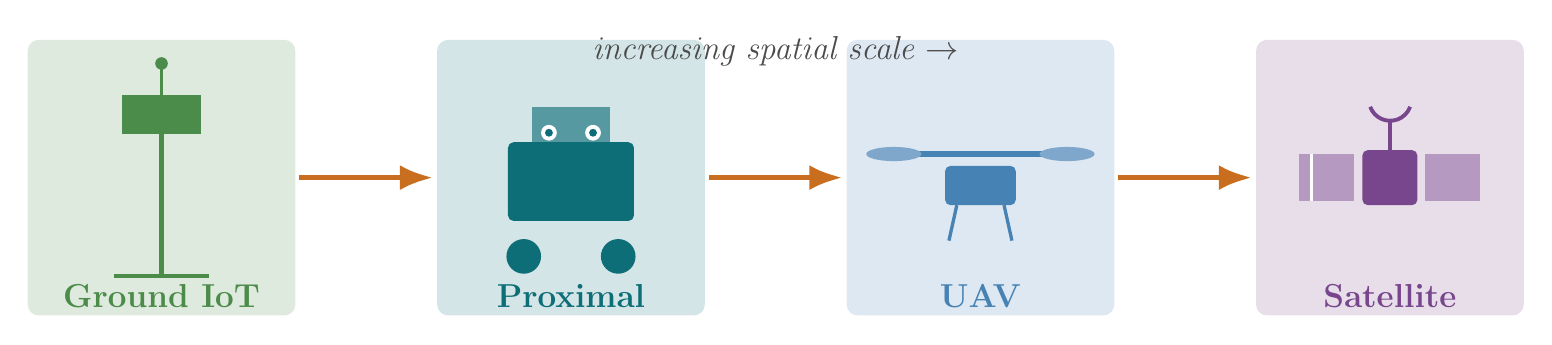
\begin{tikzpicture}[font=\sffamily, >=Latex]
\def\dx{5.2}

% ---- 1. Ground IoT (sensor post) ----
\begin{scope}[shift={(0,0)}]
  \fill[leaf!18, rounded corners=4pt] (-1.7,-1.5) rectangle (1.7,2.0);
  \draw[line width=2pt, leaf] (0,-1.0) -- (0,0.8);            % post
  \fill[leaf] (-0.5,0.8) rectangle (0.5,1.3);                  % box
  \draw[line width=1.4pt, leaf] (0,1.3) -- (0,1.7);            % antenna
  \fill[leaf] (0,1.7) circle (0.08);
  \draw[line width=1.4pt, leaf] (-0.6,-1.0) -- (0.6,-1.0);     % ground
  \node[font=\bfseries\large, color=leaf] at (0,-1.25) {Ground IoT};
\end{scope}

% ---- 2. Proximal / robot ----
\begin{scope}[shift={(\dx,0)}]
  \fill[accent!18, rounded corners=4pt] (-1.7,-1.5) rectangle (1.7,2.0);
  \fill[accent, rounded corners=2pt] (-0.8,-0.3) rectangle (0.8,0.7);  % body
  \fill[accent!70] (-0.5,0.7) rectangle (0.5,1.15);                     % head
  \fill[white] (-0.28,0.82) circle (0.10);\fill[white](0.28,0.82)circle(0.10);
  \fill[accent](-0.28,0.82)circle(0.05);\fill[accent](0.28,0.82)circle(0.05);
  \fill[accent] (-0.6,-0.75) circle (0.22);\fill[accent](0.6,-0.75)circle(0.22); % wheels
  \node[font=\bfseries\large, color=accent] at (0,-1.25) {Proximal};
\end{scope}

% ---- 3. UAV / drone ----
\begin{scope}[shift={(2*\dx,0)}]
  \fill[sky!18, rounded corners=4pt] (-1.7,-1.5) rectangle (1.7,2.0);
  \fill[sky, rounded corners=2pt] (-0.45,-0.1) rectangle (0.45,0.4);    % body
  \draw[line width=2pt, sky] (-1.1,0.55) -- (1.1,0.55);                  % arms
  \fill[sky!70] (-1.1,0.55) ellipse (0.35 and 0.09);                     % rotors
  \fill[sky!70] (1.1,0.55) ellipse (0.35 and 0.09);
  \draw[line width=1.2pt, sky] (-0.3,-0.1) -- (-0.4,-0.55);              % legs
  \draw[line width=1.2pt, sky] (0.3,-0.1) -- (0.4,-0.55);
  \node[font=\bfseries\large, color=sky] at (0,-1.25) {UAV};
\end{scope}

% ---- 4. Satellite ----
\begin{scope}[shift={(3*\dx,0)}]
  \fill[plum!18, rounded corners=4pt] (-1.7,-1.5) rectangle (1.7,2.0);
  \fill[plum, rounded corners=2pt] (-0.35,-0.1) rectangle (0.35,0.6);   % body
  \fill[plum!55] (-1.15,-0.05) rectangle (-0.45,0.55);                   % panel L
  \fill[plum!55] (0.45,-0.05) rectangle (1.15,0.55);                     % panel R
  \draw[line width=1pt,white] (-1.0,-0.05)--(-1.0,0.55);(-0.7,-0.05)--(-0.7,0.55);
  \draw[line width=1.4pt, plum] (0,0.6) -- (0,1.0);
  \draw[line width=1.4pt, plum] (-0.25,1.15) arc (200:340:0.27);         % dish hint
  \node[font=\bfseries\large, color=plum] at (0,-1.25) {Satellite};
\end{scope}

% ---- arrows between ----
\foreach \i in {0,1,2}{
  \draw[->, line width=2pt, orange] ({\i*\dx+1.75},0.25) -- ({\i*\dx+3.45},0.25);
}
% scale label under arrows
\node[font=\large\itshape, color=black!70] at (1.5*\dx,1.85) {increasing spatial scale $\rightarrow$};
\end{tikzpicture}
\end{document}
